%%%%%%%%%%%%%%%%%%%%%%%%%%%%%%%%%%%%%%%%%%%%%%%%%%%%%%%%%%%%%%%%%%%%%%%%%%%%%%%%%
%
%  Diplomarbeit Vorname Name Datum
%  "Titel"
%  Lehrstuhl fuer Mustererkennung, FAU Erlangen-Nuernberg
%
%%%%%%%%%%%%%%%%%%%%%%%%%%%%%%%%%%%%%%%%%%%%%%%%%%%%%%%%%%%%%%%%%%%%%%%%%%%%%%%%%

% ++ LME LateX Dokument
%    Die Verwendung der option "german" bindet german.sty ein.
%    For english papers, use the "english" option and talk to your advisor.
% \documentclass[german,mt]{lmedoc}
\documentclass[english,mt]{lmedoc}

% ++ Umlaut Unterstuetzung
%    Paket "inputenc" kann verwendet werden, um z.B. Umlaute oder das scharfe S
%    direkt (als Nicht-ASCII-Zeichen) einzubinden. Dabei auf die korrekte
%    Kodiermethode achten (z.B. Linux: latin1)!
\usepackage[latin1]{inputenc}
% abbrevations
\usepackage{acronym}
% for code
% to forbid tables to get repositioned on top / bot
\usepackage{float}
\restylefloat{table}

% TODO add this in the end, currently makes compilation insanely slow
% \usepackage{hyperref}
% maybe like this idk
% \usepackage[pdftex,colorlinks=true,urlcolor=refC,linkcolor=refC,citecolor=citeC]{hyperref} % math

\usepackage{amsmath}
\usepackage{amssymb}
\newcommand{\R}{\mathbb{R}}
\newcommand{\N}{\mathbb{N}}


% drawing
\usepackage{tikz}
\usetikzlibrary{decorations.pathreplacing}
\usetikzlibrary{fadings}

% graphics
\usepackage{graphicx}

% for urls in bib
\usepackage{url}

% algorithms
\usepackage{listings}
\usepackage{color}
\usepackage{caption}

\newcounter{nalg}[chapter] % defines algorithm counter for chapter-level
\renewcommand{\thenalg}{\thechapter .\arabic{nalg}} %defines appearance of the algorithm counter
\DeclareCaptionLabelFormat{algocaption}{Algorithm \thenalg} % defines a new caption label as Algorithm x.y

\lstnewenvironment{algorithm}[1][] %defines the algorithm listing environment
{
    \refstepcounter{nalg} %increments algorithm number
    \captionsetup{labelformat=algocaption,labelsep=colon} %defines the caption setup for: it uses label format as the declared caption label above and makes label and caption text to be separated by a ':'
    \lstset{ %this is the stype
        mathescape=true,
        frame=tB,
        numbers=left,
        numberstyle=\tiny,
        basicstyle=\scriptsize,
        keywordstyle=\color{black}\bfseries\em,
        keywords={,input, output, return, datatype, function, in, if, else, foreach, do, while, begin, end, for} %add the keywords you want, or load a language as Rubens explains in his comment above.
        numbers=left,
        xleftmargin=.04\textwidth,
        #1 % this is to add specific settings to an usage of this environment (for instnce, the caption and referable label)
    }
}
{}
% multiline formulas
% \usepackage{breqn}

% non-retarded new line
\newcommand{\lf}{\\[\baselineskip]}

% ++ es werden keine underfull hboxes als Fehler ausgegeben,
%    da das ja nur hei�t, dass die Seite noch nicht ganz voll ist
\hbadness=10000



\includeonly{mt01, mt02, mt03, mt04, mt05, mt06, mt07, mt08, mt09, mt10, mt11, mt-lit, mt-lof, mt-lot}

\pagenumbering{roman}

%\bibliographystyle{galpha1a} %german bibliography
\bibliographystyle{alphamod} %english bibliography

% fix bad url formatting
\usepackage{etoolbox}
\apptocmd{\thebibliography}{\raggedright}{}{}

\begin{document}
\clearpage
  \begin{deckblatt}
    \Titel{Detection of Hand Drawn Electrical Circuit Diagrams and their Components using Deep Learning Methods and Conversion into LTspice Format}
    \Name{Vinokour}
    \Vorname{Dmitrij}
    \Geburtsort{St. Petersburg}
    \Geburtsdatum{19.12.1993}
    \Betreuer{Florian Thamm M. Sc., Felix Denzinger M. Sc., Prof. Dr. Andreas Maier}
    \Start{01.01.2021}
    \Ende{31.07.2021}
  \end{deckblatt}

\cleardoublepage

Ich versichere, dass ich die Arbeit ohne fremde Hilfe und ohne Benutzung
anderer als der angegebenen Quellen angefertigt habe und dass die Arbeit
in gleicher oder "ahnlicher Form noch keiner anderen Pr"ufungsbeh"orde
vorgelegen hat und von dieser als Teil einer Pr"ufungsleistung
angenommen wurde. Alle Ausf"uhrungen, die w"ortlich oder sinngem"a"s
"ubernommen wurden, sind als solche gekennzeichnet.
\\

Die Richtlinien des Lehrstuhls f"ur Studien- und Diplomarbeiten
habe ich gelesen und anerkannt, insbesondere die Regelung des
Nutzungsrechts. \\[15mm]
Erlangen, den \selectlanguage{german} \today \hspace{6.0cm} \\[10mm]

\selectlanguage{english} %remove this line for german style

\cleardoublepage

% \makeglossary
\begin{center}
\bfseries
"Ubersicht
\normalfont
\end{center}


\vspace{5.0cm}

\begin{center}
\bfseries
Abstract
\normalfont
\end{center}

\cleardoublepage

\tableofcontents

\cleardoublepage \pagenumbering{arabic}

\chapter{Introduction}

\section{Motivation}

\section{Related Works}

The aim of this thesis is to provide a conversion pipeline for hand-drawn \acp{ECD} into the LTspice schematic file format.
To provide some context for the task, the following subsections present approaches related to the goal of this thesis.

- TODO general structure

\subsection{Classification of Eletrical Circuit Components}

G"unay et al. \cite{ecd_basecnn} compared in their work the accuracy of various common \ac{CNN} architectures trained on a dataset of hand-drawn \acp{ECC}.
The dataset consisted of four classes (resistor, capacitor, inductor, voltage source) and had overall a size of 863 images. best cnn 83\%

- fourier svm
- logical gates (AND, OR, NOT)
- segmentation of components based on closed region
- draw bbox around region
- feature extraction + svm
- 180 samples
- 83 \% accuracy

-



\section{Goals of the Thesis}

\subsection{Task Description}

\subsection{Contribution}

\cleardoublepage
\chapter{Theory}

\section{Electrical Circuit Diagrams}

An \ac{ECD} consists of \ac{ECCs} where for each \ac{ECC} an unique symbol is defined in the international standard \cite{iec60617}.
\ac{ECCs} are connected with lines, which correspond to wires in the real world.
Additionally, \ac{ECCs} are further specified by an annotation next to their symbol, which consists of a digit followed by a unit.
For instance a resistor can be denoted as ``100 m$\Omega$'' (Milliohm).

- TODO introduce more symbols?

- TODO generally create hyperref to abbrevations

- TODO sources current with arrows?

- TODO image?

\section{LTspice File}
LTspice is a circuit simulation software, where circuits can be modeled, parametrized and simulated.
A modeled circuit is stored in a LTspice schematic file, with the file extension .asc.
Since, the last step in the pipeline of this thesis is the conversion of the hand drawn \acp{ECD} into a LTspice schematic file, the file structure and syntax were analyzed and are presented in this section.

\subsection{General}
LTspice files are written in plain text and are human readable.
The file structure has to be interpreted line by line, meaning that one command is written on one line.
Inside a line a command is separated by a space.
In most cases the first word of a line is a keyword indicating the used command, which then is followed by parameters provided to the command.

LTspice itself provides a grid, where components are aligned to.
This grid has a size of $32x32$ units, where a unit is an abstract measure inside of LTspice.

\subsection{File Definition}

\subsubsection{Header}

Each schematic file starts with a header, which defines the used version of the syntax.
Throughout this thesis the forth version of the syntax is used. Table \ref{tab:ltheader_syntax} shows the syntax for the version definition command.

\begin{table}[H]
\begin{center}

\begin{tabular}{l|l|l}
    & \textbf{Keyword} & \textbf{Param1}\\
    \hline
    \textbf{Syntax} & VERSION & version number\\
    \textbf{Info} & & in this thesis 4
\end{tabular}
\caption{LTspice header syntax}
\label{tab:ltheader_syntax}

\end{center}
\end{table}


\subsubsection{Symbols}

In LTspice \acp{ECC} are called symbols.
The syntax to define a symbol is presented in table \ref{tab:ltsymbol_syntax}.
The command is declared by using the keyword ``SYMBOL'' followed by a symbol name, where the symbol name is a mapping to an \ac{ECC}.
All symbol names which are used in this thesis are shown in table \ref{tab:ltsymbol_mapping}.
The symbol name is followed by two integers defining the $x$ and $y$ coordinate of the symbol.
The coordinates are representing the upper left corner of the symbols image used to represent the symbol inside LTspice.
Additionally a rotation has to be provided with $Rr$ where $r$ defines the rotation in degree.
The rotation $r$ is constrained to be either $0$, $90$ or $270$ degree.
So an example for a resistor declaration would be: ``SYMBOL res 32 32 R90'', which means that a resistor is defined at $x = 32$, $y = 32$ with a rotation of $90$ degree.

\begin{table}[H]
\begin{center}

\begin{tabular}{l|l}
    \textbf{Electrical Circuit Component} & \textbf{LTspice keyword}\\
    \hline
    Resistor & res\\
    Capacitor & cap\\
    Inductor & ind\\
    Diode & diode\\
    Voltage Source & voltage\\
    Current Source & current
\end{tabular}
\caption{LTspice symbol names}
\label{tab:ltsymbol_mapping}

\end{center}
\end{table}

\begin{table}[H]
\begin{center}

\begin{tabular}{l|l|l|l|l|l}
    & \textbf{Keyword} & \textbf{Param1} & \textbf{Param2} & \textbf{Param3} & \textbf{Param4}\\
    \hline
    \textbf{Syntax} & SYMBOL & symbol name & X-Coordinate & Y-Coordinate & Rotation\\
    \textbf{Info} & & see table \ref{tab:ltsymbol_mapping} & multiple of 32 & multiple of 32 & R0, R90, R270
\end{tabular}
\caption{LTspice symbol syntax}
\label{tab:ltsymbol_syntax}

\end{center}
\end{table}

\subsubsection{Symbol Attributes}

A symbol can be further specified through the usage of a symbol attribute.
The symbol attribute is always applied to the first occurrence of a previously defined symbol relative to this command.
The syntax for this command is presented in table \ref{tab:ltsymattr_syntax}.
This command is declared using the keyword ``SYMATTR'' followed by the targeted attribute and the corresponding value to be set for the targeted attribute.
Two attributes can be used as a target for this command.
The ``InstName'' attribute allows to declare a name for the symbol and the value therefore is a string.
The ``Value'' attribute allows to declare a component value for the symbol always defined in the corresponding base unit of the component (e.g. $\Omega$ for resistors).

\begin{table}[H]
\begin{center}

\begin{tabular}{l|l|l|l|l|l}
    & \textbf{Keyword} & \textbf{Param1} & \textbf{Param2}\\
    \hline
    \textbf{Syntax} & SYMATTR & attribute & value\\
    \textbf{Info} & & Value, InstName & Integer, String\\
\end{tabular}
\caption{LTspice symbol attribute syntax}
\label{tab:ltsymattr_syntax}

\end{center}
\end{table}

\subsubsection{Ground}

Grounds are defined by using the keyword ``FLAG'' followed by the coordinates of the ground.
An additional ``0'' has to be placed at the end of the line, which indicates that the used flag is indeed a ground node.
Note that it was not further analyzed which effect the last parameter has on the flag definition, but it can be said that when the ``0'' is not present the ground is not defined correctly.
The syntax for grounds can be seen in table \ref{tab:ltflag_syntax}.

\begin{table}[H]
\begin{center}

\begin{tabular}{l|l|l|l|l}
    & \textbf{Keyword} & \textbf{Param1} & \textbf{Param2} & \textbf{Param3}\\
    \hline
    \textbf{Syntax} & FLAG & X-coordinate & Y-coordinate & flag indicator\\
    \textbf{Info} & & multiple of 32 & multiple of 32 & 0 for ground\\
\end{tabular}
\caption{LTspice ground syntax}
\label{tab:ltflag_syntax}

\end{center}
\end{table}

\subsubsection{Wire}

After the symbols have been defined they are connected through wires.
Wires in LTspice are defined as lines.
The syntax is presented in table \ref{tab:ltwire_syntax}.
The command begins with the keyword ``WIRE'' followed by two coordinate pairs.
The first pair is the beginning of the line and second the end of the line.

- TODO
Note that there is no constraint which point has to be first or second as long as the wire endpoint overlaps with a component it is connected.

\begin{table}[H]
\begin{center}

\begin{tabular}{l|l|l|l|l|l}
    & \textbf{Keyword} & \textbf{Param1} & \textbf{Param2} & \textbf{Param3} & \textbf{Param4}\\
    \hline
    \textbf{Syntax} & WIRE & X1-coordinate & Y1-coordinate & X2-coordinate & Y2-coordinate\\
    \textbf{Info} & & multiple of 32 & multiple of 32 & multiple of 32& multiple of 32  \\
\end{tabular}
\caption{LTspice wire syntax}
\label{tab:ltwire_syntax}

\end{center}
\end{table}


\section{Artificial Neural Networks}
\subsection{General Concepts}
\label{sec:deep_basics}

The basic building blocks of an \ac{ANN} are Artificial Neurons, which are inspired by  their biological counterparts.
Biological neurons receive a signal via dendrites and output the processed signal through the axon \cite{bioneuron}.

The first artificial neuron, the Perceptron, was proposed by Rosenblatt \cite{perceptron}.
The decision rule for the Perceptron is described by eq. \ref{form:perceptron}.
It states that the output $\hat{y} \in \{-1, 1\}$ is defined by the sign of the dot product of a weight vector $V \in \R^{n}$ with an input vector $x \in \R^{n}$.
The decision boundary of this function is a linear function, which means non-linear problems like the XOR-problem, can't be solved with the perceptron.

\begin{equation}
    \hat{y} = sign(V^Tx)
    \label{form:perceptron}
\end{equation}

\subsubsection{Multi Layer Perceptron}

To tackle this insufficiency the \ac{MLP} was introduced \cite{mlp}, which is able to solve non-linear problems.
Generally, a \ac{MLP} consists of three layer types: one input layer, one or more hidden layers and one output layer.
The input layer is the identity function (eq. \ref{eq:identity}), which forwards the input $x \in \R^n$ without change to the following hidden layer.

\begin{equation}
    I(x) = x
    \label{eq:identity}
\end{equation}

The hidden layer, which is also called a \ac{FC} layer \cite{dl} is build out of one to $m \in \N$ Perceptrons.
The output output vector $\hat{y} \in \R^m$ is calculated by multiplying $x$ with each weight vector $V \in R^n$ and adding a constant bias vector $b \in \R^m$ to the calculation \cite{dl_mit}.

\begin{equation}
    \hat{y} = (V_1^Tx, \cdots, V_m^Tx)^T + b
\end{equation}

The calculation can further be simplified by using a weight matrix, which combines all weights $V$ and the bias $b$.
The output $\hat{y}$ is then simply the matrix multiplication of the weight matrix $W \in R^{(n+1) \times m}$ with the input vector $x$.
Note that, to fit the dimensionality $x$ has to be extended with a \textit{1} at the end hence results in $x \in \R^{(n+1)}$ \cite{dl}.
The current output vector $\hat{y}$ is just a linear transformation of the input vector $x$, but biological neurons are also able to process a received signal non-linearly \cite{dl_mit}, therefore activation functions $f_{a}: \R^n \to \R^n$ are used to mimic this behavior.
Some commonly used activation functions and specifically the ones used in this thesis are presented in section \ref{sec:activation_functions}.
Combining the activation function and the matrix multiplication results in the following formula:

\begin{equation}
    \hat{y} = f_a(W^Tx)
    \label{eq:fc_weights}
\end{equation}

The last missing layer type is the output layer, which in a classification setting outputs a vector of conditional class probabilities $\hat{y} \in \R^n$, where $n$ is the number of classes.
Commonly the softmax activation function is used to produce such an output \cite{softmax}.
The softmax function takes as input the output of a previous layer and outputs a vector of pseudo probabilities by taking the fraction of the exponential function applied to an element of the input vector, divided by the sum of all exponential function outputs applied to all elements of the input vector.
A pseudo probability element in the output vector is defined as follows:

\begin{equation}
    softmax(x)_i = \frac{e^{x_i}}{\sum_{j=1}^Ne^{x_j}}
\end{equation}

Since the output of one layer is the input for the following layer a \ac{MLP} can be mathematically described in a chain like function structure as $f^{(O)}( f^{(n)} ( \cdots f^{(1)} (f^{(I)}(x))))$, where $f^{(I)}$ is the input layer, $f^{(O)}$ the output layer and $f^{(1)} \cdots f^{(n)}$ are the amount of $n$ hidden layers, respectively.

\begin{figure}[t]
	\centering
	\begin{tikzpicture}[shorten >=1pt]
		\tikzstyle{unit}=[draw,shape=circle,minimum size=1.15cm]
		\tikzstyle{hidden}=[draw=none]
        \tikzstyle{weight}=[draw,shape=rectangle,minimum size=0.6cm]


        % input layer
        \node[unit](b0) at (0, 7, 0){$1$};
        \node[unit](x1) at (0, 5, 0){$x_1$};
        \node[unit](x2) at (0, 3, 0){$x_2$};
        \node at (0, 1.5){\vdots};
        \node[unit](xn) at (0, 0, 0){$x_n$};
		\draw [decorate,decoration={brace,amplitude=10pt},xshift=-4pt,yshift=0pt] (-0.5,8) -- (0.75,8) node [black,midway,yshift=+0.6cm]{input layer};

        % weight layer
        \node[weight](w00) at (2, 7.5, 0){$w_{0,0}$};
        \node[weight](w01) at (2, 6.5, 0){$w_{0,1}$};

        \node[weight](w10) at (2, 5.5, 0){$w_{1,0}$};
        \node[weight](w11) at (2, 4.5, 0){$w_{1,1}$};

        \node[weight](w20) at (2, 3.5, 0){$w_{2,0}$};
        \node[weight](w21) at (2, 2.5, 0){$w_{2,1}$};

        \node[weight](wn0) at (2, 0.5, 0){$w_{n,0}$};
        \node[weight](wn1) at (2, -0.5, 0){$w_{n,0}$};

        % sum layer
        \node[unit](sum0) at (5, 5, 0){$\Sigma$};
        \node[unit](sum1) at (5, 2, 0){$\Sigma$};

        % activation layer
        \node[unit](acti0) at (7, 5, 0){$f(x)$};
        \node[unit](acti1) at (7, 2, 0){$f(x)$};
		\draw [decorate,decoration={brace,amplitude=10pt},xshift=-4pt,yshift=0pt] (6.5,6) -- (7.75,6) node [black,midway,yshift=+0.6cm]{activation function};

		\draw [decorate,decoration={brace,amplitude=10pt},xshift=-4pt,yshift=0pt] (1.5,8) -- (7.75,8) node [black,midway,yshift=+0.6cm]{1. layer};

        % weight layer 2
        \node[weight](w200) at (9, 5, 0){$w_{0,0}$};
        \node[weight](w201) at (9, 2, 0){$w_{0,1}$};

        % sum layer 2
        \node[unit](sum2) at (11, 3.5, 0){$\Sigma$};

        % activation layer 2
        \node[unit](acti2) at (13, 3.5, 0){$f(x)$};
		\draw [decorate,decoration={brace,amplitude=10pt},xshift=-4pt,yshift=0pt] (12.5,4.5) -- (13.75,4.5) node [black,midway,yshift=+0.6cm]{activation function};


		\draw [decorate,decoration={brace,amplitude=10pt},xshift=-4pt,yshift=0pt] (8.5,8) -- (13.75,8) node [black,midway,yshift=+0.6cm]{2. layer};

        % hidden output
        \node[hidden](h0) at (15, 3.5, 0){};

        \draw[->](b0) -- (w00);
        \draw[->](b0) -- (w01);

        \draw[->](x1) -- (w10);
        \draw[->](x1) -- (w11);

        \draw[->](x2) -- (w20);
        \draw[->](x2) -- (w21);

        \draw[->](xn) -- (wn0);
        \draw[->](xn) -- (wn1);

        \draw[->](w00) -- (sum0);
        \draw[->](w10) -- (sum0);
        \draw[->](w20) -- (sum0);
        \draw[->](wn0) -- (sum0);

        \draw[->](w01) -- (sum1);
        \draw[->](w11) -- (sum1);
        \draw[->](w21) -- (sum1);
        \draw[->](wn1) -- (sum1);

        \draw[->](sum0) -- (acti0);
        \draw[->](sum1) -- (acti1);

        \draw[->](acti0) -- (w200);
        \draw[->](acti1) -- (w201);

        \draw[->](w200) -- (sum2);
        \draw[->](w201) -- (sum2);

        \draw[->](sum2) -- (acti2);
        \draw[->](acti2) -- (h0);

	\end{tikzpicture}
	\caption{Multi Layer Perceptron with two layers}
	\label{fig:mlp}
\end{figure}


% The \ac{MLP} is created by using the output of multiple perceptrons as an input to another perceptron.
% In fig. \ref{fig:mlp} the general structure of a \ac{MLP} is shown.
% This particular \ac{MLP} has two neurons in the first layer and one in the second layer.
% In general the number for neurons inside a layer, as the number of layers is not bounded.

\subsubsection{Learning Procedure}

In the first step the input data is fed to the network producing an output $\hat{y}$.
This step is called forward propagation and is just the above described method of calculating the output of a layer and using it as the input for the next one.

Afterwards, the output $\hat{y} \in \R^n$ is compared to the desired output $y \in \R^n$ using a loss function $L(y, \hat{y}): (\R^n, \R^n) \to \R$.
A common loss function is the \ac{MSE} \cite{yolov1}, which calculates the mean sum of the squared differences between the inputs $y$ and $\hat{y}$ (eq. \ref{eq:mse}).

\begin{equation}
    \label{eq:mse}
    MSE(y, \hat{y}) = \frac{1}{n} \sum_{i=1}^{n}(y_i - \hat{y}_i)^2
\end{equation}

Another common example of a loss function would be the \ac{CE} Loss (eq. \ref{eq:ce}), which measures the difference between two probability distributions for a given random variable or a set of events. \cite{loss_function_segmentation}

\begin{equation}
    \label{eq:ce}
    CE(y, \hat{y}) =
    \begin{cases}
        -log(\hat{y}), & \text{if } y = 1\\
        -log(1 - \hat{y}), & \text{else}
    \end{cases}
\end{equation}

The resulting loss value is used to calculate the gradients with respect to the last layer weights. Due to the above described chained function structure of an \ac{MLP} the chain rule can be used to propagate the error back through the network and calculate the gradients for all remaining layers.

After all gradients have been calculated the weights of each layer are optimized.
A simple optimizer is the stochastic gradient descent, whose update rule is defined as:

\begin{equation}
    w^{(k+1)} = w^{(k)} - \eta \nabla L(w^{(k)})
\end{equation}

Here, $w^{(k+1)}$ denotes the updated weights, and $w^{(k)}$ the current state of the weights.
$\eta$ is the learning rate of the network, which is essentially the amount of the gradient which should be used to update the weights.
Typically an $0 < \eta < 1$ is chosen, since big values have shown to make the training process unstable, resulting in divergence of the loss.
Further, $\nabla L(w^{(k)})$ should denote here the gradients with respect to the loss function at the respective layer.

To accelerate the training the stochastic gradient descent can be extended by a momentum term \cite{sgd_momentum}.
The momentum term and the resulting update rule are defined as follows:

\begin{equation}
    v^{(k)} = \mu v^{(k-1)} - \eta \nabla L(w^{(k)})
\end{equation}

\begin{equation}
    w^{(k+1)} = w^{(k)} + v^{(k)}
\end{equation}

$\mu$ denotes here the momentum value which is typically set to $0.9$, $0.99$ respectively \cite{adam}.
The idea is that one can incorporate the weighted value of the previous update, to accelerate in directions with persistent gradient \cite{dl}.

\subsection{Activation Functions}
\label{sec:activation_functions}

Non-linear activation functions play a crucial role in the performance of an \ac{ANN}, since this enables function approximation \cite{mish}.
In the Perceptron the \textit{sign} function was used, but due to its non-differentiable property it isn't suited for the use in \acp{ANN}, since back propagation requires differentiability of the activation function.
Therefore, various differentiable activation functions have been introduced.

\subsubsection{Sigmoid}

The sigmoid activation function (eq. \ref{eq:sigmoid}) is a smooth differentiable activation function, which maps its input to a $\{0, 1\}$-space.
It is commonly used in output layers, since the output of the sigmoid can be interpreted as a probability.
A major drawback of the sigmoid lies in the saturating property for $x \to \pm \infty$, when it's used as an activation function in trainable layers of \acp{ANN}.
Due to this the training process suffers from the so called vanishing gradient problem, where the derivative of the sigmoid tends to go towards zero and hence does not provide an update to the weights of the \ac{ANN}.

\begin{equation}
    \sigma(x) = \frac{1}{1 + e^{-x}}
    \label{eq:sigmoid}
\end{equation}

\subsubsection{Rectified Linear Unit (ReLU)}

The \ac{ReLU} activation function solves the gradient vanishing problem by introducing a linear term for input values $x > 0$, while maintaining the non-linearity property by setting all negative input values to $0$.
The \ac{ReLU} activation function is defined as follows:

\begin{equation}
    ReLU(x) =
    \begin{cases}
        x, & \text{if } x > 0\\
        0, & \text{else}
    \end{cases}
\end{equation}

A variation of the \ac{ReLU} activation function is the \ac{LReLU} activation function, where additionally negative values are scaled linearly.
\ac{LReLU} was introduced to tackle the dying \ac{ReLU} problem, where the network only predicts negative values and hence all gradients become zero \cite{dl}.
It is defined as follows:

\begin{equation}
    LReLU(x) =
    \begin{cases}
        x, & \text{if } x > 0\\
        \alpha x, & \text{else}
    \end{cases}
\end{equation}

% \subsubsection{ReLU6}

% ReLU6 is a modification of the classical \ac{ReLU}, where the output activation is limited to 6.
% It is often used in resource constrained environments, especially in cases of low precision computation, since it has shown to perform robust in such cases. \cite{mnetv1}

% \begin{equation}
%     ReLU6(x) =
%     \begin{cases}
%         6, & \text{if } x >= 6\\
%         x, & \text{if } 0 < x < 6\\
%         0, & else
%     \end{cases}
% \end{equation}

% \subsubsection{Hard Swish}

% Hard Swish \cite{mnetv3} is an approximation of the original Swish activation function, which was discovered by the researchers at Google in their extensive search for novel activation functions \cite{swish}.
% Hard Swish is calculated by multiplying the input with a piece-wise linear sigmoid approximation, the Hard Sigmoid (eq. \ref{eq:hard_sigmoid}).
% As with ReLU6, Hard Swish is used in resource constrained environments.

% \begin{equation}
%     Swish_{hard}(x) = x \sigma_{hard}(x)
% \end{equation}

% \begin{equation}
%     \sigma_{hard}(x) = \frac{ReLU6(x + 3)}{6}
%     \label{eq:hard_sigmoid}
% \end{equation}


\subsection{Convolutional Neural Networks}

While \acp{MLP} perform pretty well on vectorial data, multidimensional data like images for example, can only be fed to a network when it was previously flattened into a vector.
One problem that arises is that when flattening for example an image of size $100 \times 100$, this would already require the input size of the network to have $10.000$ weights per neuron in the next layer.
Additionally nearby pixels in images are often highly correlated and classical unstructured \ac{ANN} fails to capture such spatial dependencies. \cite{lecun_lenet}

The proposed alternative therefor are \acp{CNN}, which have shown to perform pretty well over the last decade in several image related benchmarks. \cite{inception} \cite{resnet} \cite{densenet}.
The classical \ac{CNN} architecture is comprised of three different layer types: convolutional layers, pooling layers and fully-connected layers.

\subsubsection{Convolutional Layer}
Convolutional layers form the major component in a \ac{CNN}.
As the name suggest the underlying mathematical foundation of those layers is the convolution operation.
The equation for a convolution (eq. \ref{eq:conv}), states that a function $f$ convolved with another function $g$, is the multiplication of those two functions, while $g$ is shifted over $f$.
The final result is then obtained by taking the integral over the whole domain. \cite{dl}

\begin{equation}
    (f * g)(x) = \int_{-\infty}^{\infty}f(\tau)g(x - \tau)d\tau
    \label{eq:conv}
\end{equation}

In simpler terms that just means there is an image $I \in \R^{WxHxC}$, where $W$ and $H$ are the width and height of the image and $C$ being the number of channels.
Further, there is a kernel $K \in \R^{W_KxH_KxC}$.
The image and the kernel are now convolved by moving the kernel over the image and at each position an element-wise multiplication of the overlapping area of the image and the kernel is taken.
Afterwards, the result is summed up and used as an output element in the convolution result.
Finally, the kernel is shifted further until the whole image has been processed.
How much pixel a kernel is shifted at a time depends on the used stride.
The higher the stride the less local information is preserved.
Typically a stride of $1$ or $2$ is used.
An example of a convolution of a $4\times4$ input with a $3\times3$ kernel and a stride of $1$ is given in figure \ref{fig:conv_example}.

\begin{figure}
\begin{center}
    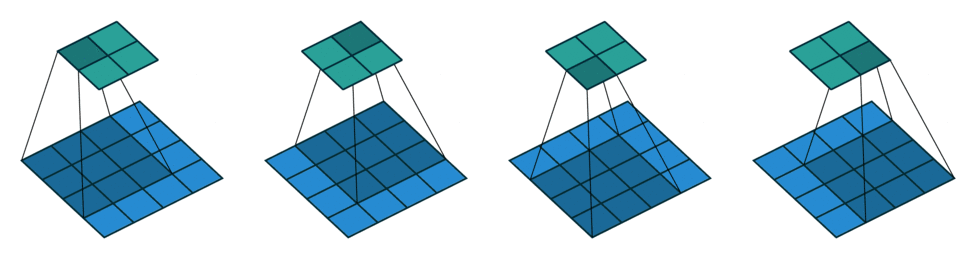
\includegraphics[width=16cm]{imgs/conv_example_full.png}
    \caption{Example convolution of a 4x4 input (blue) with a 3x3 kernel (dark blue) and a stride of 1, resulting in a 2x2 output (cyan) \cite{conv_arithmetic}}
    \label{fig:conv_example}
\end{center}
\end{figure}

\subsubsection{Pooling Layer}
\label{sec:max_pooling}

Pooling layers in \acp{CNN} are used to further reduce the dimensionality of the output.
During the pooling operation information across spatial locations is fused by sliding a window (typically of size $2\times2$ or $3\times3$) over the input and performing a function on the values inside the window.
In the case of max pooling the used function is the $MAX$ function, therefore only the maximum value inside the window is considered and used in the pooling output.
This decreases the number of parameters and hence reduces the computational cost. \cite{dl}

\subsubsection{Fully-Connected Layer}

The \ac{FC} layer as described in \ref{sec:deep_basics} is the final layer inside a \ac{CNN}.
The high-level features, which were previously build through the convolutional and max pooling layers, are flattened into a fixed size vector and passed for classification to the \ac{FC} layer.

\subsection{Batch Normalization}

A common problem while training with the \ac{ReLU} activation function is that the outputs are non-zero centered, since \ac{ReLU} is non-zero centered.
So with each layer the output distribution gets shifted from the input distribution.
This observed phenomenon is called the \textit{internal co-variate shift} and forces the network to adapt to the shifting output distribution.
The adaption produces an overhead, which is expressed in a longer training time of the network.
Therefore, Ioffe and Szegedy \cite{batchnorm} introduced \ac{BatchNorm}, a trainable layer for \ac{ANN}.
The \ac{BatchNorm} layer normalizes the feature maps along the batch axis to have zero-mean and a standard deviation of one, which not only decreases the training time, but also allows for higher learning rates and less careful initialization of the network weights.


\section{Data Augmentation}

\section{Object Detection}
\label{sec:object_detection}

Object detection is one of the subtasks in the image domain.
It is an extension of the classification task, where additionally to the predicted class, the location of the objects in the image should be predicted.
The location is normally given as a bounding box, where throughout this thesis the bounding box format by Redmon et al. \cite{yolov1} is used to label object instances.
In this format a bounding box is defined as:

\begin{equation}
    bbox = (x_{rel}, y_{rel}, w_{rel}, h_{rel})
\end{equation}

Where the bounding box is presented as a tuple of four values.
The first two values indicate the center of the bounding box relative to the image size, while the latter two values indicate the width and the height of the bounding box also relative to the image size.
All values can be calculated by dividing the absolute value by the corresponding image value.
For example $x_{rel}$ would be calculated by dividing the absolute x-coordinate $x_{abs}$ by the width of the image.
Same applies for $y_{rel}$, except here the value is divided by the image height.
$w_{rel}$ and $h_{rel}$ are calculated following the same principles.
The advantages of this format are, that the definition of the bounding box becomes invariant to the image size.
The image can be resized without having to recalculate the bounding box, as it is the case with other formats which use an absolute definition for bounding boxes.

\subsection{History of Object Detection}
\label{sec:hostory_obj_detection}

\subsubsection{Sliding Window}
The simplest algorithm to detect objects in an image is the sliding window approach.
A classifier is trained on image patches which contain the object to detect.
To now detect the objects in an unseen image, the image is divided into patches of various scale and fed to the classifier.
The prediction score of the patches is thresholded with a predefined value.
High confidence patches are likely to contain an object and are kept \cite{sliding_window_satelite}.

% Before an object detection can be performed on an image, a classifier has to be trained.
% This classifier is normally trained on image patches, where a patch has roughly the size of the objects it should classify.
% The object detection phase starts by dividing the input image into patches.
% Those patches are now fed to the classifier and when the predicted probability exceeds a predefined threshold the patch is considered to have an object in it.
% It should be noted that classification accuracy can be improved by feeding overlapping patches into the classifier.
% The resulting predicted bounding boxes now look like the image on the left side in fig. \ref{fig:nms_before_after}.
% It contains multiple bounding boxes for the same object.
% To have only one prediction per object, a \ac{NMS} algorithm is applied on the overlapping bounding boxes.
% The most common \ac{NMS} algorithm is the greedy-\ac{NMS}.
% Here bounding boxes are grouped together, when their overlap exceeds a certain threshold.
% Rejection of neighboring bounding boxes is done by using the predicted class probability i.e. using only those bounding boxes with the highest prediction score and rejecting the others \cite{learn_nms}.
% The results of a \ac{NMS} can be seen on the right side in fig. \ref{fig:nms_before_after}.


% - TODO add tackle scale by using patches of different size

% \begin{figure}
% \begin{center}
%     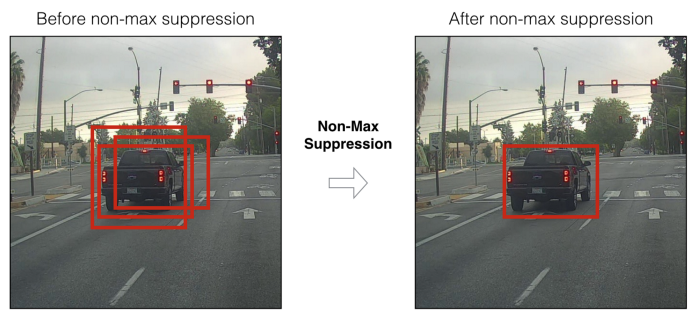
\includegraphics[width=10cm]{imgs/nms_before_after.png}
%     \caption{Predicted bounding boxes before and after a non-maximum suppression was applied \cite{nms_before_after}}
%     \label{fig:nms_before_after}
% \end{center}
% \end{figure}

\subsubsection{Regions with CNN Features (R-CNN)}
While the sliding window approach is effective, it is also highly inefficient, since every generated patch has to be processed by the classifier in order to find all possible objects in an image.
\ac{R-CNN} by Girshick et al. \cite{rcnn} improves on that by using a region proposal algorithm to obtain probable regions of an object.
In their work the Selective Search algorithm \cite{selective_search} was used to generate region proposals.
How the algorithm performs and what kind of bounding boxes are produced, can be seen in fig. \ref{fig:selective_search}.
$2000$ of those proposed bounding boxes are taken from different scales and warped into the input shape of the following \ac{CNN}, disregarding the size or aspect ratio of the proposed bounding box.
Each of the bounding boxes is separately passed through the \ac{CNN} and yields a feature vector which is classified by $N + 1$ binary \acp{SVM} ($N$ classes $+1$ general background class) to produce the class prediction.
Further, the bounding box is improved through $N$ separately trained bounding box regressor \acp{SVM} \cite{bbox_regressor}.

\begin{figure}
\begin{center}
    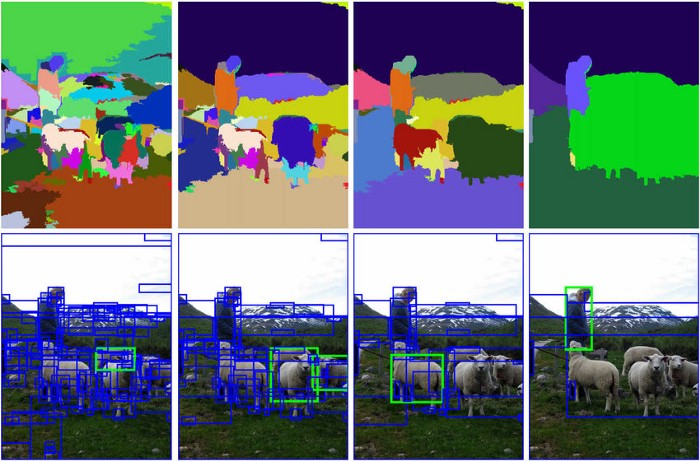
\includegraphics[width=10cm]{imgs/selective_search.png}
    \caption{Example of results obtained through the Selective Search algorithm (top) with increasing region scale from left to right and bounding boxes drawn around those regions (bottom). Selective Search produces sub-segmentations of objects in an image, considering size, color, texture and shape based features for the grouping of the regions \cite{selective_search}.}
    \label{fig:selective_search}
\end{center}
\end{figure}

\subsubsection{Fast R-CNN}
While \ac{R-CNN} was an improvement to the previous methods, the training and inference process was still very expensive, since it involved multiple stages.
With Fast R-CNN Girshick \cite{fast_rcnn} improved on the training and inference time by a large margin in contrast to \ac{R-CNN}.

The main difference to \ac{R-CNN} is that instead of generating region proposals and passing them through the \ac{CNN}, region proposals are now projected onto the feature maps of the \ac{CNN} and pooled into a fixed size grid through a \ac{RoI} pooling layer.
Meaning that the \ac{CNN} computations are shared between each bounding box proposal resulting in a drastic inference speed improvement.
After pooling, the \ac{RoI} it is processed by a fully-connected layer, producing a so called \ac{RoI} feature vector.
This feature vector is fed into a siblings output layer.
The first branch is a classification layer with a softmax output, producing class probabilities and replaces the previous \acp{SVM}.
The second branch is comprised of a bounding box regression layer, which outputs bounding box regression offsets as in \ac{R-CNN} \cite{rcnn}.
% Due to the one-stage nature of the pipeline a novel multi-task loss was required,
% which the author defined as follows:

% \begin{equation}
%     L(\hat{y}, y, \hat{b}, b) = L_{cls}(\hat{y}, y) + \lambda L_{loc}(\hat{b}, b)
% \end{equation}

% $\hat{y}$ being the predicted class probabilities by the softmax layer and $y$ the ground truth class.

% - TODO should I even do that further?

% \subsubsection{Faster R-CNN}

% In Fast \ac{R-CNN} the prediction time was decreased by compressing the multi-stage pipeline into a single-stage pipeline.
% The remaining non-learnable part of the pipeline became the region proposal algorithm.
% It still took around $2s$ to propose bounding boxes with Selective Search.
% Ren et. al therefore proposed Faster \ac{R-CNN} \cite{faster_rcnn} to further increase the performance of the overall algorithm.
% In Faster \ac{R-CNN} the performance is boosted through the novel \ac{RPN}.
% As with Fast \ac{R-CNN} an image is first fed to the \ac{CNN} to produce feature maps.
% Afterwards, the feature maps are used as an input to the \ac{RPN}, which operates in a sliding window fashion, where a window size of $nxn$ ($n = 3$) is used to traverse the whole feature map and produce features for the following network.

\subsubsection{Anchor Box Based Single Shot Detectors}

Various object detection networks such as, Faster \ac{R-CNN} \cite{faster_rcnn}, \ac{YOLO} \cite{yolov1}, \ac{SSD} \cite{ssd} and RetinaNet \cite{focalloss} use anchor boxes to predict the objects in an image.
Further, all the named methods predict the class as well as the bounding boxes for the objects in a single network pass, therefore the name single shot.
Anchor boxes are predefined boxes of various size aspect ratio, which are used as a base for the prediction bounding box prediction of the above networks.
Instead of making the network predict the bounding box directly, the network predicts bounding box regression offsets based on a certain anchor box \cite{yolov3}.
The selection of good anchor box sizes is a hyperparameter in the training of an object detector and can improve the prediction quality \cite{faster_rcnn}.
The scale and aspect ratio of the anchor boxes is often selected by using the k-means clustering algorithm on the labeled bounding boxes of the dataset \cite{yolov2}.


% Anchor boxes are used to assign a ground truth to a prediction of a network, which is then used to apply a loss on the prediction and hence make the network learn.
% For example in Faster \ac{R-CNN} the ground truth bounding box is assigned to an anchor when the \ac{IoU} of the bounding box and the anchor box is greater than a certain threshold.
% Anchor boxes can be seen as predictors, who over time get better and better of predicting objects of certain size and aspect ratios \cite{yolov1}.


\subsubsection{Anchor Box Free Single Shot Detectors}

Another class of single shot detectors are the anchor box free detectors such as \ac{YOLOv1} \cite{yolov1}, CornerNet \cite{corner_net}, CenterNet \cite{center_net} and the \ac{FCOS} \cite{fcos}.
The advantages of anchor box free detection methods are that complicated computation related to anchor boxes, e.g. calculating the \ac{IoU} at training time, can be omitted \cite{fcos}, as well as the tuning of anchor box sizes for the specific task \cite{center_net}.
As of now, all the above methods perform worse than their current state-of-the-art anchor box based counterparts \cite{yolov4}.



\subsection{Intersection Over Union (IoU)}

The \ac{IoU}, which is also known as the Jaccard index, is a measure for how much two arbitrary shapes (volumes) are overlapping \cite{giou}.
In object detection \ac{IoU} is often used to compare two bounding boxes $A$ and $B$ and also to construct various loss functions as well as metrics.

\begin{equation}
    \text{IoU}(A, B) = \frac{|A \cap B|}{|A \cup B|} = \frac{| A \cap B |}{|A| + |B| - |A \cap B|}
\end{equation}


\subsection{IoU Based Loss Functions}

The \ac{MSE} has shown to perform not well for the task of bounding box regression, because it assumes that the regressed variables ($x$, $y$, $w$, $h$) are independent of each other and can be optimized separately \cite{iou}.

To take the correlation of those variables into account, Yu et al. \cite{iou} proposed the \ac{IoU} loss (equation \ref{eq:iou_loss}).
While this was a major improvement to previously known methods the \ac{IoU} loss still suffers from slow convergence and from the gradient vanishing problem, which occurs when the two bounding boxes $A$ and $B$ have no intersection.

\begin{equation}
    \text{L}_{\text{IoU}}(A, B) = 1 - \text{IoU}(A, B)
    \label{eq:iou_loss}
\end{equation}

Further, to solve these drawbacks Rezatofighi et al. \cite{giou} proposed the \ac{GIoU} loss (equation \ref{eq:giou_loss}).
Their loss introduces an additional penalty term added to the \ac{IoU} loss.
Here, $C$ is the smallest convex box enclosing $A$ and $B$.
Hence, when the boxes have no overlap there is still a gradient pushing them closer to each other.
While the \ac{GIoU} loss is a major improvement in terms of vanishing gradient, it suffers from slow convergence when $A$ and $B$ have overlap and at the same time $A$ contains $B$ (or vice versa), because the penalty term then becomes $0$, as a consequence the \ac{GIoU} loss becomes the \ac{IoU} loss.
Furthermore, it has been observed that when $A$ and $B$ have no overlap, instead of decreasing the spatial distance between $A$ and $B$, the \ac{GIoU} loss tends to increase the size of the bounding box area to reduce the loss \cite{eiou}.

\begin{equation}
    \text{L}_{\text{GIoU}}(A, B) = 1 - \text{IoU}(A, B) + \frac{|C - (A \cup B)|}{|C|}
    \label{eq:giou_loss}
\end{equation}

The next improvement in the \ac{IoU} based loss function space was proposed by Zheng et al. \cite{diou}, with their \ac{DIoU} and \ac{CIoU} loss functions.
In contrast to \ac{GIoU}, \ac{DIoU} (equation \ref{eq:diou_loss}) solves the gradient vanishing problem by considering the normalized distance of the central points of the two bounding boxes.
The squared euclidean distance is normalized by the squared diagonal length of the smallest box containing $A$ and $B$.

\begin{equation}
    \text{L}_{\text{DIoU}}(A, B) = 1 - \text{IoU}(A, B) + \frac{\|(A_{center} - B_{center})\|^2}{\|C_{diag}\|^2}
    \label{eq:diou_loss}
\end{equation}

To further improve on that, the authors additionally considered the aspect ratio of the bounding box to be another important geometric factor for bounding box regression.
Hence, the \ac{DIoU} loss is further extended by a penalty term considering the aspect ratio and resulting in the improved \ac{CIoU} loss (equations \ref{eq:ciou_loss}, \ref{eq:ciou_nu}, \ref{eq:ciou_alpha}).

The penalty in \ac{CIoU} is split into $\alpha$ and $\nu$.
The term $\alpha$ is a trade-off parameter which gives higher priority to the overlapping factor, especially in the case of non-overlap.
Further, $\nu$ is the parameter penalizing the difference in the aspect ratios of $A$ and $B$.
Still, it can be noticed that $\nu$ is $0$ when the aspect ratios are the same, regardless of the underlying relations between $A_w$, $B_w$ and $A_h$, $B_h$.
E.g. the aspect ratio is the same for all boxes with the following property $\{ (A_w=kB_w, \ A_h=kB_h)\ |\ k \in \R^+\}$ \cite{eiou}.

\begin{equation}
    \text{L}_{\text{CIoU}}(A, B) = \text{DIoU}(A, B) + \alpha(A,B) \cdot \nu(A, B)
    \label{eq:ciou_loss}
\end{equation}

\begin{equation}
    \nu(A, B) = \frac{4}{\pi^2} \left[arctan\left(\frac{A_w}{A_h}\right) - arctan\left(\frac{B_w}{B_h}\right)\right]^2
    \label{eq:ciou_nu}
\end{equation}

\begin{equation}
    \alpha(A, B) = \frac{\nu}{1 - IoU(A, B) + \nu'}
    \label{eq:ciou_alpha}
\end{equation}

Therefore, Zhang et al. \cite{eiou} proposed the \ac{EIoU} loss to remove this error.
The aspect ratio penalty is here replaced through two separate penalties, which consider the normalized width and height of the two bounding boxes.

\begin{equation}
    \text{L}_{\text{EIoU}}(A, B) = 1 - IoU(A, B) + \frac{\|(A_{center} - B_{center})\|^2}{\|C_{diag}\|^2} + \frac{\|(A_{w} - B_{w})\|^2}{\|C_w\|^2} + \frac{\|(A_{h} - B_{h})\|^2}{\|C_h\|^2}
    \label{eq:eiou_loss}
\end{equation}


\section{Segmentation}
\label{sec:segmentation}

Segmentation is another subtask in the image domain.
The target here is to obtain a mask of an object or objects in an image.
It is related to the classical classification problem, but instead of predicting the class for a whole image, the class is here predicted for each pixel individually.
Segmentation can be further divided into semantic segmentation \cite{semantic_segmentation} and instance segmentation \cite{mask_rcnn}.
In semantic segmentation the type of an object in general is predicted for example cat or dog.
In instance segmentation further the instance of an object is predicted so, e.g. when two cats are present two separate masks would be predicted.
Figure \ref{fig:instance_vs_semantic} illustrates the two different types of segmentation.

\begin{figure}
\begin{center}
    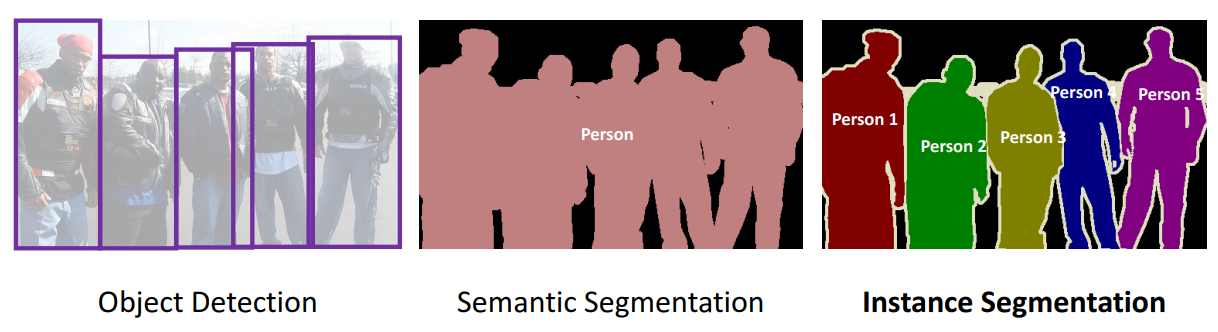
\includegraphics[width=16cm]{imgs/instance_vs_semantic_seg.png}
    \caption{The difference between object detection, semantic segmentation and instance segmentation. In object detection the instance with a rough estimate (bounding box) is predicted, in semantic segmentation a segmentation mask for an object is predicted without considering the underlying instance and in instance segmentation the instance as well as a segmentation mask for an object is predicted. \cite{instance_vs_semantic_fig}}
    \label{fig:instance_vs_semantic}
\end{center}
\end{figure}

\section{MobileNetV2-UNet}
\label{sec:mobilenetv2_unet}

For the segmentation of the circuits \ac{MUnet} \cite{mobile_unet} is used.
This network is build upon the principles of the famous U-Net proposed by Ronneberger et al. \cite{unet}.
The classical U-Net architecture consists of two main components: an encoder and a decoder.
The encoder is a classical \ac{CNN} which learns the features of the provided data.
It uses convolutional layers and max pooling layers to downsample the feature map size.
The decoder does the inverse, here the feature maps are convolved and then upsampled.
Which made the U-Net unique at the proposed time is that to enhance the segmentation results, additionally after a feature map was upsampled it gets concatenated with a feature map from the backbone which has the same resolution.
It should be noted that this approach was probably picked up by the \ac{YOLOv4} developers and reused in their architecture as has been shown in section \ref{sec:yolo}.

\ac{MUnet} is a combination of the MobileNetV2 \cite{mnetv2} which is used as the backbone and a decoder which is adapted to the backbone.
In the following section the architecture of the \ac{MUnet} is explained.

\subsubsection{MobileNetV2-UNet backbone}

MobileNetV2 is the backbone of the \ac{MUnet} and can be decomposed into two main components:

\begin{itemize}
    \item depthwise separable convolutions
    \item inverted residual blocks
\end{itemize}

Depthwise separable convolutions were already used in the first MobileNet and are a way to factorize a standard convolution into a depthwise convolution and a $1\times1$ convolution.
Essentially this means that a classical convolution is split into two layers, in the depthwise convolutional layer first a convolution is applied on each channel separately, i.e. given an input $I \in \R^{H \times W \times C}$ and $C$ kernels $K^{h \times w \times 1}$ each channel $C_i$ is convolved with a corresponding kernel $K_i$.
Afterwards, to build up features lightweight $1 \times 1$ convolutions are used.
This method has shown to perform almost on par with a classical convolution, but reduces the amount of computation by a factor of eight \cite{mnetv1}.
Hence, this method is perfectly suited for resource constrained environments such as mobile phones.

The inverted residual layer is a novel layer in MobileNetV2.
The idea is to first project the input feature maps into a lower dimensional subspace by using a $1 \times 1$ convolution with ReLU6 non-linearity, the resulting feature maps are then expanded inside the block by a following depthwise separable convolution.
Afterwards, the output is again convolved with $1 \times 1$ convolution.
Further, the inverted residual has a residual connection where the input is added to the output of the last linear $1 \times 1$ convolution.
The whole inverted residual block can be seen in figure \ref{fig:inverted_residual} it also shows that the input gets expanded inside the inverted residual block.
The expansion factor $t \in \N$ defines how much the input is expanded inside the inverted residual block.
The expansion can be seen in table \ref{tab:invres_expansion}.

\begin{table} %[H]
\begin{center}

\begin{tabular}{l|l|l}
\textbf{Input} & \textbf{Operator} & \textbf{Output}\\
\hline
$h \times w \times k$ & $1 \times 1$ conv2d, BatchNorm, ReLU6 & $h \times w \times (tk)$\\
$h \times w \times (tk)$ & $3 \times 3$ dwise s=s, BatchNorm, ReLU6 & $\frac{h}{s} \times \frac{w}{s} \times (tk)$ \\
$\frac{h}{s} \times \frac{w}{s} \times (tk)$ & $1 \times 1$ conv2d, BatchNorm & $\frac{h}{s} \times \frac{w}{s} \times k'$
\end{tabular}

\caption{An inverted residual block transforming from $k$ to $k'$ channels, with stride $s$ and expansion factor $t$.}
\label{tab:invres_expansion}
\end{center}
\end{table}

\begin{figure}
\begin{center}
    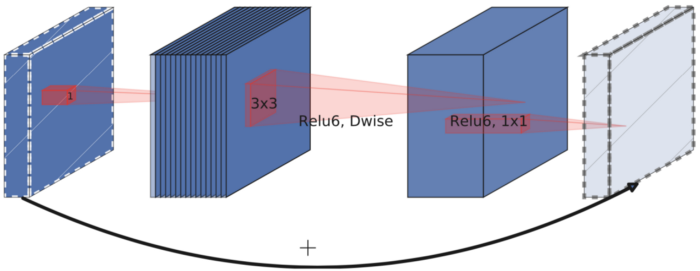
\includegraphics[width=13cm]{imgs/inverted_residual.png}
    \caption{The inverted residual block. A $1 \times 1$ convolution with non-linear activation followed by a depthwise separable convolution and a linear $1 \times 1$ convolution with residual connection to the input. The residual connection is here additive, i.e. the input gets added to the output of the linear $1 \times 1$ convolution.}
    \label{fig:inverted_residual}
\end{center}
\end{figure}

% The development of this layer was guided by the important factors that feature maps are able to be encoded in low-dimensional subspaces and that the use of \ac{ReLU} can result in information loss if input features are not embedded in a low-dimensional subspace \cite{mnetv2}.
% So the idea behind the layers is when first the input features get embedded into a low-dimensional subspace

The whole MobileNetV2 architecture is given in table \ref{tab:mobilenetv2_architecture}.

\begin{table} %[H]
\begin{center}

\begin{tabular}{l|l|l|l|l|l|l|l}
\textbf{Blocks} & \textbf{Operation} & \textbf{t} & \textbf{k} & \textbf{n} & \textbf{s} & \textbf{Output (h, w, c)}\\
\hline
Input           & -             & - & - & - & - & (448, 448, 3) \\
                & Conv+BN+ReLU6 & - & 3 & 1 & 2 & (224, 244, 32) \\
$Skip_{1}$      & InvRes        & 1 & - & 1 & 1 & (224, 224, 16)\\
$Skip_{2}$      & InvRes        & 6 & - & 2 & 2 & (112, 112, 24) \\
$Skip_{3}$      & InvRes        & 6 & - & 3 & 2 & (56, 56, 32) \\
                & InvRes        & 6 & - & 4 & 2 & (28, 28, 64) \\
$Skip_{4}$      & InvRes        & 6 & - & 3 & 1 & (28, 28, 96) \\
                & InvRes        & 6 & - & 3 & 2 & (14, 14, 160) \\
                & InvRes        & 6 & - & 1 & 1 & (14, 14, 320) \\
$Skip_{5}$      & Conv+BN+ReLU6 & - & 1 & - & - & (14, 14, 1280) \\
\end{tabular}

\caption{MobileNetV2 backbone used in \ac{MUnet} Blocks marked as $Skip_*$ are outputs from the network which are used in the decoder. The parameters above define the configuration of the respective block, $t$ is the expansion factor inside an inverted residual block as defined in \ref{tab:invres_expansion}, $k$ is the kernel size for the two standard convolutions used in the backbone, $n$ defines how often that particular block is repeated and $s$ is the stride of a block. Note that if $s = 2$ only the first block has this stride, the others have $s = 1$.}
\label{tab:mobilenetv2_architecture}
\end{center}
\end{table}

\subsubsection{MobileNetV2-UNet decoder}

The decoder of \ac{MUnet} is build by the principles of U-Net\cite{unet}.
Feature map upsampling is done using transposed convolutions.
After a feature map has been upsampled it is concatenated with a skip connection from the backbone with the same spatial dimension.
Concatenation is performed along the channel axis.
To unify the novel concatenated feature map it is passed to a inverted residual block.
This step is repeated until no skip connections from the backbone are left.
The last step in the decoder is composed of a bilinear upsampling layer, which is used to produce a prediction which has the same size as the input image.
This has to be done because the backbone directly downsamples the image size in the first layer and hence there is no feature map with the same spatial dimensions as the input image.
The architecture of the backbone can be found in table \ref{tab:mobilenetv2_decoder}.

\begin{table} %[H]
\begin{center}

\begin{tabular}{l|l|l|l|l|l|l|l}
\textbf{Block} & \textbf{Inputs} & \textbf{Operation} & \textbf{t} & \textbf{k} & \textbf{s} & \textbf{Output (h, w, c)}\\
\hline
$Up1$     & $Skip_5$        & ConvTranspose & - & 4 & 2 & (28, 28, 96) \\
$InvRes1$ & $Skip_4 + Up1$  & InvRes        & 6 & - & 1 & (28, 28, 96) \\
$Up2$     & $InvRes1$       & ConvTranspose & - & 4 & 2 & (56, 56, 32) \\
$InvRes2$ & $Skip_3 + Up2$  & InvRes        & 6 & - & 1 & (56, 56, 32) \\
$Up3$     & $InvRes2$       & ConvTranspose & - & 4 & 2 & (112, 112, 24) \\
$InvRes3$ & $Skip_2 + Up3$  & InvRes        & 6 & - & 1 & (112, 112, 24) \\
$Up4$     & $InvRes3$       & ConvTranspose & - & 4 & 2 & (224, 224, 16) \\
$InvRes4$ & $Skip_1 + Up4$  & InvRes        & 6 & - & 1 & (224, 224, 2) \\
$Up5$     & $InvRes4$       & UpBillinear   & - & - & 2 & (448, 448, 2) \\
\end{tabular}

\caption{\ac{MUnet} decoder. The decoder uses transpose convolutions to upsample the input (ConvTranspose) and as the backbone, inverted residuals to process the upsampled input together with the skip connection. The '+' indicates a concatenation along the channel axis. Since the first block in the backbone directly downsamples the input there is no skip connection with the size of the input. Therefore the last layer of the decoder is a upsampling layer, which uses a bilinear upsampling method to increase the size of the prediction to the size of the input. As with the backbone $t$ indicates the expansion size of the inverted residual block, $k$ indicates the used kernel size and $s$ indicates the used stride.}
\label{tab:mobilenetv2_decoder}
\end{center}
\end{table}


\section{Connected Components Analysis}
- TODO write why I need CCA?

- TODO later

A \ac{CCA} describes the process of labeling connected pixels in a binary image.

In the most simple case a structuring element such as a cross (four-connection-labeling) or a rectangle (eight-connection-labeling) is moved over an image and if two pixels are neighbors and their value is the same they are considered to have the same label. In this thesis the eight-connection-labeling algorithm by Grana et al. \cite{cca} is used.


\section{Optical Character Recognition}

\section{Hypergraphs}


\section{Metrics}

\cleardoublepage
\chapter{Material and Methods}

\section{Data}
The images of \acp{ECD} were acquired throughout the thesis.
The


\section{Recognition and Conversion Pipeline}
\label{sec:pipeline}

In this section the pipeline is presented, which allows to convert an image of an \ac{ECD} into the LTspice schematic file format.
To fully convert the \ac{ECD} from the \ac{IDom} into the \ac{LDom} the following needed conditions have been identified:

\begin{itemize}
    \item the class and position of the \acp{ECC}
    \item the text and position of the annotations as well as the annotation mapping (to which \ac{ECC} belongs this annotation)
    \item the connections between the \acp{ECC}
    \item the conversion into the LTspice schematic file
\end{itemize}

The above points are all embedded into a three-stage pipeline, which will be presented throughout this section.

\subsubsection{Recognition}

Predicting the class and position of an object can essentially be formulated as an object detection problem.
Various object detection networks exist, which could be used for this task.
In this thesis the presented \ac{YOLOv4}-Tiny (section \ref{sec:yolo}), or just \ac{YOLO} is used to predict the \acp{ECC}, \ac{ECC}-annotations (arrows for sources) and the text annotations in the \ac{IDom}.
\ac{YOLO} was chosen since it has a good compromise between network size and classification performance.

Furthermore, the pipeline also utilizes segmentation to segment the circuit.
Segmentation is needed because the topology building step, which will be described next requires a clean mask of the circuit.
The initial clean mask was created using image binarization.
While the topology building worked for circuits with white background it failed for circuits with checkered background.
Therefore, the \ac{MUnet} (section \ref{sec:mobilenetv2_unet}) is used to segment a circuit in the \ac{IDom}.
The network predicts a binary classification output in the form background / not background, where everything which is unrelated to the \ac{ECD} is considered background.
Note that the network was trained for both checkered and uncheckered backgrounds, such that it can be applied on both types of images.
Again, \ac{MUnet} was chosen, since it is a lightweight network with appropriate performance, able to be used on mobile devices.

An example prediction of both networks can be seen in figure \ref{fig:example_predictions}.

\begin{figure}
\begin{center}
    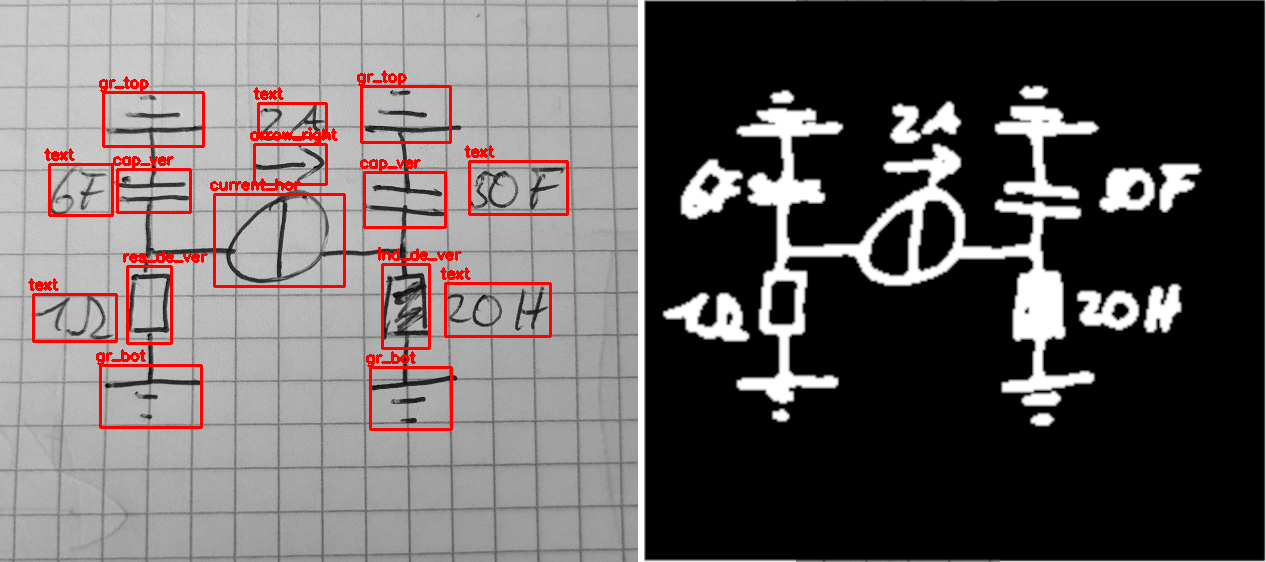
\includegraphics[width=16cm]{imgs/pipeline/combined_pred.png}
    \caption{Example predictions of YOLO (left) and \ac{MUnet} (right). YOLO predicts a bounding box around each component with its corresponding class, while \ac{MUnet} predicts a segmentation mask a binary fashion of the whole \ac{ECD} drawing, including \ac{ECC} annotations. Primary segmentation is needed to remove the checkered background from the image.}
    \label{fig:example_predictions}
\end{center}
\end{figure}

\subsubsection{Topology Creation}

The next step in the pipeline is the identification of the connections between the \acp{ECC}, such that the wires from the \ac{IDom} can be transformed into the \ac{LDom}.
In an abstract form this is topology creation.
This step does not take into account the spatial positions of the components, but only the semantics of the circuit.
In the following the algorithm is presented, which takes as input the predicted bounding boxes and the segmentation mask of the circuit and produces the topology of the circuit.
The algorithm utilizes various OpenCV algorithms, which are first briefly explained.

\textbf{Adaptive Binary Thresholding} TODO? maybe I won't use it any more

\textbf{Connected Components Labeling} by Grana et al. \cite{cca} is an 8-way connectivity algorithm used to label blob like regions in a binary image.
In the topology creation process it is used to identify the wires.

\textbf{Morphological Operations} like erosion, dilation or the combinations of those like opening and closing \cite{cv}, are used to filter the used binary images and to refine results obtained from various sources in the pipeline.

After the basic methods were presented now the algorithm can be explained.
The algorithm receives as input the predicted bounding boxes and the segmentation mask of the circuit.

\begin{enumerate}
    \item Copy the \textbf{SegmentationMask} $\in \{0,1\}^{h \times w}$  into \textbf{WiresOnly}. Iterate over the bounding boxes (bbox $\in \{x1, y1, x2, y2, class\}$, where $(x1, y1)$ represent the upper left corner of the bounding box and $(x2, y2)$ the lower right) and remove every pixel in \textbf{WiresOnly}, which is included in a bounding box. Only the wires remain now.
    \item Perform morphological closing on \textbf{WiresOnly} to close up small holes in the wires.
    \item Apply connected components labeling on \textbf{WiresOnly} to label the separate wire blobs resulting in \textbf{WiresLabeled}.
    \item Create a matrix \textbf{BBoxMask} of zeros with the size of \textbf{WiresOnly}. Iterate over the bounding boxes and populate \textbf{BBoxMask} with rectangles with a thin border created from the bounding box coordinates.
    \item Apply the and-operator on \textbf{WiresLabeled} and \textbf{BBoxMask} and receive the intersections, where a wire is intersecting the border of a bounding box. Store the result in \textbf{Intersections}.
    \item Initialize a dictionary \textbf{Topology} and populate it by iterating over \textbf{Intersections} and for each intersection index check the connected components label at this index create an entry in \textbf{Topology} with an empty array.
    \item Iterate over each intersections index and find the bounding box which is ``involved'' in this intersection. A bounding box is ``involved'', when intersection index $\in$ bounding box border and the class of the bounding box is an \ac{ECC}.
    \item Find the orientation of the intersection. Orientation refers to the connection orientation relative to the bounding box, i.e. is the intersection at the top, bottom, left or right border.
    \item Get the connected components label at the intersection index and add a tuple of (bounding box index, orientation) at the respective spot in the \textbf{Topology} if this index with this orientation is not present.
    \item After the initial \textbf{Topology} is build, iterate over it and remove each connected component label, where the involved bounding boxes array has $size = 1$ and the involved bounding box has a contradictory orientation in relation to the predicted class, i.e. classes predicted with vertical orientation can only have a connection at the top or bottom, classes predicted with horizontal orientation can only have a connection left or right.
    \item Return the \textbf{Topology}
\end{enumerate}

\subsubsection{Annotation Matching}

In this thesis different annotations are used.
Arrow annotations are only used for voltage and current sources to indicate the direction of the potential difference as well as the current flow, respectively.
On the other side textual annotations can be applied to any type of an \ac{ECC}.
To fully reflect the circuit in the \ac{LDom} annotations have to be matched against their respective \ac{ECC}.
The algorithm used in this thesis is presented in algorithm \ref{alg:annotation_matching}, it takes as input a list of arrow bounding boxes, a list of text bounding boxes and a list of \acp{ECC}.
An annotation is matched against an \ac{ECC} using a simple brute force nearest neighbor approach, based on the center distance of the bounding boxes to match.
Brute force in the sense that every annotation will get matched against an \ac{ECC} without considering that the distance between annotation and \ac{ECC} is maybe way too big, like it would be the case for example when a \ac{FP} annotation is predicted, it certainly will get matched.
Multiple annotations are also possible with this algorithm, but when this occurs the one with the smallest distance is taken and the other match is ignored.

\begin{algorithm}[caption={Annotation Matching TODO caption to bottom and format}, label={alg:annotation_matching}]
input:  $A = \{a_1, ..., a_n\}$, $T = \{t_1, ..., t_m\}$, $E = \{e_1, ..., e_o\}$
        $A$: list of predicted arrow bounding boxes
        $T$: list of predicted text bounding boxes
        $E$: list of predicted ECC bounding boxes
output: $A_m = \{(a_1, e_i), ..., (a_n, e_j)\}$
        $T_m = \{(t_1, e_x), ..., (t_m, e_y)\}$
        $A_m$: list of arrow bounding boxes matched against source bounding boxes
        $T_m$: list of text bounding boxes matched against ECC bounding boxes

begin
    $A_m = \{\}$
    foreach $a$ in $A$; do
        $distances = \{\}$

        $a_{center}$ = get_bounding_box_center($a$)
        foreach $e$ in $E$; do
            if is_source_type($e$); then
                $e_{center}$ = get_bounding_box_center($e$)
                $dist$ = euclidean_distance($a_{center}$, $e_{center}$)
                $distances$ $\gets$ $distances + (dist, a, e)$
            end
        end

        $min_{dist}$, $a_{matched}$, $e_{matched}$ = sort_ascending_by_distance($distances$)[0]
        $A_m = A_m \gets (a_{match}, e_{match})$
    end

    $T_m = \{\}$
    foreach $t$ in $T$; do
        $distances = \{\}$

        $t_{center}$ = get_bounding_box_center($t$)
        foreach $e$ in $E$; do
            $e_{center}$ = get_bounding_box_center($e$)
            $dist$ = euclidean_distance($t_{center}$, $e_{center}$)
            $distances$ $\gets$ $distances + (dist, t, e)$
        end

        $min_{dist}$, $t_{matched}$, $e_{matched}$ = sort_ascending_by_distance($distances$)[0]
        $T_m = T_m \gets (t_{match}, e_{match})$
    end

    return $A_m$, $T_m$
end
\end{algorithm}


\subsubsection{LTspice Conversion}

The last step in the proposed pipeline is the embedding of the gathered information into the LTspice schematic file.

TODO not 100\% sure how this will be written


\cleardoublepage
\chapter{Pipeline Evaluation}

This chapter presents the evaluation of the pipeline as a whole system.
First, the used evaluation algorithms are briefly explained together.
In addition also the notions of \ac{TP}, \ac{FP} and \ac{FN} are presented in their respective context.
For object detection this has already been explained in section \ref{sec:tpfpfn}.
Afterwards, the results are presented together with a thorough evaluation.

\section{Evaluation Algorithm}
\label{sec:eval_algo}

\subsubsection{Classification Evaluation}

The evaluation of the \ac{YOLO} network was already done in section \ref{sec:training}  based on the \ac{mAP} metric.
This metric considers multiple \ac{IoU} thresholds in its calculation and provides a general detection performance.
However, in the context of topology generation, a prediction with a bad \ac{IoU} with its ground truth could still lead to a correct prediction of the topology.
Therefore, for the evaluation of the full pipeline matching of bounding box predictions is done using a fixed \ac{IoU} threshold.
To find an initial guess of the threshold, first the maximum occlusion \ac{IoU} was obtained from the test dataset, by calculating the \ac{IoU} between each ground truth in an image.
The maximum occurring \ac{IoU} was found at 10\%, means that in general the dataset has low occlusion.
Under the assumption that the size of the predicted bounding boxes will be greater than the size of the respective ground truth bounding boxes the \ac{IoU} was chosen to be bigger than the maximum occlusion \ac{IoU}.
For the evaluation the \ac{IoU} threshold was hence set to 30\%.
Furthermore, for the evaluation in the section the predictions are provided with the \acp{TP}, \acp{FP} and \acp{FN} values, as well as with metrics, which can be calculated from those.

The segmentation outcome is not further quantified, but it can be said that, a bad segmentation result will be reflected in the results of the topology, which will probably have a lot of errors.

\subsubsection{Topology Evaluation}

The similarity of the predicted and the ground truth topology is measured, based a hypergraph adjacency matrix, where the format has been defined in section \ref{sec:hypergraph_topology}.
To recall, a hypergraph is defined as: $H = \{V, E\}$, with the vertices $V \in \{v_1,...,v_n\}$ and the edges, $E = \{e_1,...e_n\} = \{\{v_i,...,v_j\},...,\{v_x,...,v_y\}\}$.
Further, a subedge and the amount of subedges present in an hyperedge is defined as: $S(e_i) = \{ \{v_1,v_2\}\ |\ \{v_1,v_2\} \in e_i,\ e_i \in E\}$, $\#S(e_i) = \{ \#e_i - 1\ |\  e_i \in E\}$, where \# is the length operator for a set.

\acp{TP} in the used algorithm are always measured through a perfect match, where a perfect match occurs, when the two hyperedges (which are sets of vertices) are the same.
The amount of \acp{TP} which occurs through a perfect match is defined as amount of subedges $\#S(e_i)$ on the ground truth hyperedge.
Note, that in an error free context (no \acp{FN}, no \acp{FP}), the amount of \acp{TP} is equal to the amount of all possible predictions.

After all initial perfect matches have been identified the algorithm tries to find the remaining \acp{TP}, \acp{FP} and \acp{FN}.
Compared to object detection a \ac{FN} occurs, when a prediction is missing, i.e. a ground truth could not be matched to a prediction, since no such prediction exists.
In the context of topology matching a \ac{FN} is defined as ``a subedge is missing''.
Consider the following example:

\begin{itemize}
    \item Ground truth $H$: $V = \{v_1, v_2, v_3\}$, $E = \{\{v_1, v_2, v_3\}\}$
    \item Predicted $\hat{H}$: $\hat{V} = \{v_1, v_2, v_3\}$, $\hat{E} = \{\{v_1, v_2\}, \{v_3\}\}$
\end{itemize}

As mentioned all \ac{TP} calculations are only performed with perfect matches.
In this case a perfect match can be recreated by combining the two hyperedges in $\hat{H}$.
The resulting perfect match would have $TPs = 2$, because this is the amount of subedges $\#S(e_i)$, however actually there was one \ac{FN} since the perfect match could only be produced through recombination of predicted hyperedges.
Therefore, the notion of \acp{FN} is introduced, which are defined as:

\begin{equation}
    FNs = \#(recombined\ hyperedges\ for\ perfect\ match) - 1
    \label{eq:fns}
\end{equation}

It has been mentioned, that in an error free context the amount of \acp{TP} is equal to the amount of all possible predictions.
Further, the amount of all possible predictions is in general defined as:

\begin{equation}
    \#(all\ possible\ predictions) = TPs + FNs
    \label{eq:tps_plus_fns}
\end{equation}

Hence, the amount of \acp{TP} has to be adapted based on the amount of \acp{FN}.
Therefore, when a recombination case occurs, formula \ref{eq:tps_plus_fns} has to be used to subtract the amount of \acp{FN} from the \acp{TP}.
Resulting here in $TPs = 1$, $FNs = 1$.

Naturally the equations \ref{eq:fns} and \ref{eq:tps_plus_fns} extend to the case, where the hyperedges of $\hat{H}$ are $\hat{E} = \{\{v_1\}, \{v_2\}, \{v_3\}\}$.
Again, to have a perfect match all hyperedges have to be recombined, therefore: $FNs = 2$, $TPs = 0$.

The next case considers \acp{FP}, where a \ac{FP} is defined as: ``a subedge too much''.
Consider again the following example of a ground truth and predicted hypergraph:

\begin{itemize}
    \item Ground truth $H$: $V = \{v_1, v_2, v_3\}$, $E = \{\{v_1, v_2\}, \{v_3\}\}$
    \item Predicted $\hat{H}$: $\hat{V} = \{v_1, v_2, v_3\}$, $\hat{E} = \{\{v_1, v_2, v_3\}\}$
\end{itemize}

A \ac{FP} can be identified in general when: $e_i \subset \hat{e_j}$.
The algorithm here then removes the ground truth hyperedge from the predicted hyperedge, by setting all values in the predicted hyperedge to 0.
The remaining parts of the predicted hyperedge are then again reused for the recombination.

The algorithm in general looks like this:

\begin{enumerate}
    \item Input: ground truth hypergraph $H$, prediction hypergraph $\hat{H}$
    \item Initial Perfect Matching: Find all perfect matches between $H$ and $\hat{H}$, store perfectly matched hyperedges in \textbf{Matched}.
    \item Recombination: Try to find perfect matches with unmatched hyperedges of $H$ and $\hat{H}$, where an unmatched hyperedge is one which is not present in \textbf{Matched}.
    Use also recombination of hyperedges in $\hat{H}$ to find perfect matches and store perfectly matched hyperedges in \textbf{Matched}.
    \item Splitting: Try to find perfect matches with unmatched hyperedges of $H$ and $\hat{H}$, by trying to find an $\hat{e_i} \in \hat{E}$, where an $e_j \in E$, $e_j \subset e_i$.
    Store only $e_j$ in \textbf{Matched}.
    \item Repeat Recombination and Splitting until all hyperedges are matched.
\end{enumerate}

At the current state, the algorithm is not able to handle mixed cases of \ac{FP} and \ac{FN} such as:

\begin{itemize}
    \item Ground truth $H$: $V = \{v_1, v_2, v_3, v_4\}$, $E = \{\{v_1, v_2\}, \{v_3, v_4\}\}$
    \item Predicted $\hat{H}$: $\hat{V} = \{v_1, v_2, v_3, v_4\}$, $\hat{E} = \{\{v_1, v_3\}, \{v_2, v_4\}\}$
\end{itemize}

Here, neither through recombination, nor through splitting a perfect match can be identified.
When this occurs all the remaining unmatched ground truth hyperedges are used and the worst case scenario is computed, which is that all possible remaining \acp{TP} become \acp{FN}.

Furthermore, the algorithm also doesn't handle transient error cases in the topology evaluation.
For example when you consider that an \ac{ECC} was not predicted, at the moment that \ac{ECC} is inserted such that it is at least possible that a perfect match occurs.


\subsubsection{Annotation Matching Evaluation}

To recreate the full topology in the \ac{LDom} the textual as well as, the arrow annotations have to be matched against their respective \ac{ECC}.
Hence, part of the evaluation is to quantify the amount of correctly and falsely matched annotations.
The format of the matching labels and the matching algorithm, were already presented in section \ref{sec:data} and section \ref{sec:pipeline}, respectively.
Consider again the three possible cases for a \ac{TP}, \ac{FN} and \ac{FP}.
A \ac{TP} being the simplest case, occurs when an annotation is matched to its respective \ac{ECC}.
Further, a \ac{FN} is always a transient error from the YOLO recognition, i.e. an annotation could not be predicted and hence there exists no annotation, which can be matched against an \ac{ECC}.
The last case being the \ac{FP} case, which occurs when an annotation was matched with a wrong \ac{ECC}.

\section{Results}
\label{sec:evaluation_results}

\subsubsection{Classification}
First the results for the plain classification based on the \ac{YOLO} network are presented.
The used networks were the tuned networks from figure \ref{fig:yolo_tuning_combined_results}, while in this figure the tuning increased the overall \ac{mAP}, now the results are presented for an \ac{IoU} threshold of 0.3 as plain \ac{TP}, \ac{FP} and \ac{FN} (table \ref{tab:yolo_classification_res}).

\begin{table}[H]
\footnotesize
\begin{center}
\begin{tabular}{|l|l|l|l|l|l|l|l|l|l|l|}

\hline
\textbf{NMS} & \textbf{ScoreThr.} & \textbf{IoUThr.} & \textbf{InputSize} & \textbf{Vote} & \textbf{TP}  & \textbf{FP} & \textbf{FN} & \textbf{Precision} & \textbf{Recall}  & \textbf{F1}       \\
\hline
DIoU    & 0.3        & 0.25     & $608 \times 608$   & -     & 798 & 6  & 9  & 99.25\%   & 98.88\% & 99.07\%  \\
\hline
DIoU    & 0.3        & 0.25     & $736  \times 736$      & -     & 799 & 8  & 8  & 99.01\%   & 99.01\% & 99.01\%  \\
\hline
DIoU    & 0.15       & 0.45     & $736  \times 736$     & -     & 801 & 12 & 6  & 98.52\%   & 99.26\% & 98.89\%  \\
\hline
WBF     & 0.15       & 0.25     & $736  \times 736$      & -     & 801 & 12 & 6  & 98.52\%   & 99.26\% & 98.89\%  \\
\hline
WBF-TTA & 0.1        & 0.45     & $736  \times 736$      & 1     & 804 & 30 & 3  & 96.40\%   & 99.63\% & 97.99\%  \\
\hline
WBF-TTA & 0.1        & 0.45     & $736  \times 736$        & 2     & 804 & 21 & 3  & 97.45\%   & 99.63\% & 98.53\%  \\
\hline
WBF-TTA & 0.1        & 0.45     & $736  \times 736$        & 3     & 804 & 17 & 3  & 97.93\%   & 99.63\% & 98.77\%  \\
\hline
WBF-TTA & 0.1        & 0.45     & $736  \times 736$        & 4     & 804 & 13 & 3  & 98.41\%   & 99.63\% & 99.01\%  \\
\hline
WBF-TTA & 0.1        & 0.45     & $736  \times 736$        & 5     & 803 & 13 & 4  & 98.41\%   & 99.50\% & 98.95\%  \\
\hline

\end{tabular}
\caption{The results of the YOLO classification for the tuned networks presented in section \ref{sec:training_yolo}. Classification was done based on a matching \ac{IoU} threshold of 0.3.}
\label{tab:yolo_classification_res}
\end{center}
\end{table}

Comparing the results based on the f1-score shows, that actually the baseline (first configuration) performed best.
Increasing the input size added one \ac{TP}, but also increased the amount of \acp{FP} by two.
The further tuning of the \ac{DIoU}-\ac{NMS} and of the \ac{WBF} algorithm also led to an increase of two \acp{TP}, but also in a higher increase of \acp{FP}.
Adding \ac{TTA} shows that, the amount of \acp{TP} could be further increased, but again the trade-off is here higher increase in \acp{FP} vs. some increase in \ac{TP}.
The small gain by adding \ac{TTA} can be explained, with the observations of \cite{when_tta_works}, they showed in their experiments, that \ac{TTA} has especially a positive effect on networks, which are not well trained.
Networks, which are trained well with enough data, as it seems to be the case here, actually started to perform worse when \ac{TTA} was used.
With the addition of the proposed voting mechanism in section \ref{sec:training_yolo}, the amount of \acp{TP} can be maintained, while the amount of \acp{FP} can be decreased.
So having a voting based exclusion approach, seems to work on the test dataset.

\subsubsection{Topology}

The next presented results, are the results of the topology recognition.
To have a comparable baseline the topology first was tested with the ground truth of the \ac{YOLO} and the ground truth of the \ac{MUnet}.
Further, the baseline \ac{YOLO} from table \ref{tab:yolo_classification_res} was used to recognize the components.
Since the evaluation of the topology currently does not consider transient errors from the \ac{YOLO} recognition, the evaluation could also be performed with the ground truth, but it could be that the bounding box sizes heavily differ from the ground truth, so to make the evaluation as realistic as possible a trained \ac{YOLO} is used instead of the ground truth.
Further, the evaluation was performed for all \ac{MUnet} networks from table \ref{tab:munet_selected_nets}.

The results of the topology evaluation can be found in table \ref{tab:topology_test_plain}, where the results are listed based on the fold configuration and the learning rate.
The first listed network is the network, which was evaluated with both network ground truths.
It can be observed that the evaluation with the ground truth still had 47 \acp{FN}, which are related to either mixed cases of \ac{FP} and \ac{FN}, as described in the evaluation algorithm section \ref{sec:eval_algo}, or to false negatives produced, due to holes in the wire escaping the morphological closing.
However, it overall shows the best performance over all networks with 620 \acp{TP}.

In general it showed that all networks had a low amount of \acp{FP} (max. 7).

The fold trained with a batch size of 32 and the focal loss with an $\alpha$ of 0.1, shows generally an increase in \acp{TP} with decreasing learning rate and the smallest learning rate $1.0e^{-4}$ performed best.
When looking at the metrics why this network was selected (table \ref{tab:munet_selected_nets}), it can be seen that this network had scored best on three metrics (recall full, f1-score checkered, recall checkered).
This fold with the same loss function, but a batch size of 64, shows comparable performance, but the smallest learning rate was slightly better with one \ac{TP} more.
Interestingly the smallest learning rate was selected based on the same criteria as the networks with a batch size of 32.

The focal loss fold with an $\alpha$ of 0.8 and a batch size of 32 shows again that the higher learning rates had worse performance than the lower learning rates.
The best performing learning rate was $2.5e^{-4}$, where this network was selected best on the best f1-score on the checkered dataset.
Further, this loss function with a batch size of 64 showed the same results.
Higher learning rates perform worse than lower ones.
The best performing learning rate here was $5.0e^{-4}$ and was selected based on the best f1-score on the checkered dataset.

The last folds being the ones trained with the dice loss.
First consider the fold with a batch size of 32.
The biggest learning rate performs here not well and the smallest exceptionally bad too.
The smallest learning rate wasn't even able to reach half the performance of the other networks.
The best network in that fold and actually overall the best, had a learning rate of $1.0e^{-3}$ with 531 \acp{TP}.
This network was - as most of the others, which performed well - selected based on the best f1-score on the checkered validation set.
The last remaining fold being the one with the dice loss and a batch size of 64.
The smallest learning rate again showed very poor performance and could not reach half the performance of all other networks.
Further, the two best performing learning rate was $2.5e^{-3}$, which is also the second best performing learning rate overall with 521 \acp{TP}.
It was selected based on the best precision on the full validation set.


To summarize the presented results:
\begin{itemize}
    \item Bigger learning rates showed in general a worse performance than smaller learning rates
    \item The smallest learning rates for the focal loss folds showed the best performance for those folds ($5.0e^{-4}$, $2.5e^{-4}$, $1.0e^{-4}$).
    \item Dice loss is exceptionally sensitive to the used learning rate and the smallest learning rates showed exceptionally bad performance.
    \item The dice loss folds had the two best performing learning rates overall ($2.5e^{-3}$, $1.0e^{-3}$)
    \item Most of the best performing networks were selected based on the best f1-score on the checkered validation set.
\end{itemize}


\begin{table}
\footnotesize
\begin{center}
\begin{tabular}{|l|l|l|l|l|l|l|l|l|l|l|}

\hline
\textbf{Batch Size} & \textbf{Loss}      & \textbf{Learning Rate} & TP  & FP & FN  & Precision & Recall  & F1      \\
\hline
Ground Truth        &                    &                        & 620 & 0  & 47  & 100.0\%   & 92.95\% & 96.35\% \\
\hline
32                  & focal $\alpha=0.1$ & $1.0e^{-2}$            & 482 & 7  & 185 & 98.57\%   & 72.26\% & 83.39\% \\
\hline
32                  & focal $\alpha=0.1$ & $2.5e^{-3}$            & 488 & 4  & 179 & 99.19\%   & 73.16\% & 84.21\% \\
\hline
32                  & focal $\alpha=0.1$ & $1.0e^{-4}$            & 504 & 6  & 163 & 98.82\%   & 75.56\% & 85.64\% \\
\hline
64                  & focal $\alpha=0.1$ & $1.0e^{-2}$            & 464 & 7  & 203 & 98.51\%   & 69.57\% & 81.55\% \\
\hline
64                  & focal $\alpha=0.1$ & $5.0e^{-3}$            & 492 & 6  & 175 & 98.80\%   & 73.76\% & 84.46\% \\
\hline
64                  & focal $\alpha=0.1$ & $2.5e^{-3}$            & 491 & 4  & 176 & 99.19\%   & 73.61\% & 84.51\% \\
\hline
64                  & focal $\alpha=0.1$ & $1.0e^{-4}$            & 505 & 7  & 162 & 98.63\%   & 75.71\% & 85.67\% \\
\hline
32                  & focal $\alpha=0.8$ & $5.0e^{-3}$            & 485 & 5  & 182 & 98.98\%   & 72.71\% & 83.84\% \\
\hline
32                  & focal $\alpha=0.8$ & $2.5e^{-3}$            & 469 & 5  & 198 & 98.95\%   & 70.31\% & 82.21\% \\
\hline
32                  & focal $\alpha=0.8$ & $2.5e^{-4}$            & 498 & 5  & 169 & 99.01\%   & 74.66\% & 85.13\% \\
\hline
32                  & focal $\alpha=0.8$ & $1.0e^{-4}$            & 484 & 5  & 183 & 98.98\%   & 72.56\% & 83.74\% \\
\hline
64                  & focal $\alpha=0.8$ & $1.0e^{-2}$            & 492 & 5  & 175 & 98.99\%   & 73.76\% & 84.54\% \\
\hline
64                  & focal $\alpha=0.8$ & $1.0e^{-3}$            & 499 & 5  & 168 & 99.01\%   & 74.81\% & 85.23\% \\
\hline
64                  & focal $\alpha=0.8$ & $5.0e^{-4}$            & 511 & 4  & 156 & 99.22\%   & 76.61\% & 86.46\% \\
\hline
64                  & focal $\alpha=0.8$ & $1.0e^{-4}$            & 496 & 5  & 171 & 99.00\%   & 74.36\% & 84.93\% \\
\hline
32                  & dice               & $1.0e^{-2}$            & 449 & 5  & 218 & 98.90\%   & 67.32\% & 80.11\% \\
\hline
32                  & dice               & $5.0e^{-3}$            & 468 & 6  & 199 & 98.73\%   & 70.16\% & 82.03\% \\
\hline
32                  & dice               & $1.0e^{-3}$            & 531 & 4  & 136 & 99.25\%   & 79.61\% & 88.35\% \\
\hline
32                  & dice               & $1.0e^{-4}$            & 183 & 6  & 484 & 96.83\%   & 27.44\% & 42.76\% \\
\hline
64                  & dice               & $5.0e^{-3}$            & 457 & 6  & 210 & 98.70\%   & 68.52\% & 80.88\% \\
\hline
64                  & dice               & $2.5e^{-3}$            & 521 & 5  & 146 & 99.05\%   & 78.11\% & 87.34\% \\
\hline
64                  & dice               & $1.0e^{-3}$            & 512 & 5  & 155 & 99.03\%   & 76.76\% & 86.49\% \\
\hline
64                  & dice & $1.0e^{-4}$            & 185 & 6  & 482 & 96.86\%   & 27.74\% & 43.12\% \\
\hline

\end{tabular}
\caption{Results of the topology evaluation. The focal loss folds all have $\gamma = 2$. The used networks were the ones selected in table \ref{tab:munet_selected_nets}.}
\label{tab:topology_test_plain}
\end{center}
\end{table}

\subsubsection{Arrow and Text Matching}

The last step in the evaluation of the whole pipeline is composed of an evaluation of the matching algorithm \ref{alg:annotation_matching} for the text and arrow annotations.
The evaluation of the matching does not depend on the segmentation and is therefore only shown for the networks shown in table \ref{tab:yolo_classification_res}.

Table \ref{tab:text_matching_results} shows the results of the text matching, where all configurations showed the same results.
Every text annotation, which also had to be matched against an \ac{ECC} was predicted, therefore the results have no \acp{FN}.
The only error source were here \acp{FP}, which were produced either due to a \ac{FP} prediction of the \ac{YOLO} network, hence being a transient error, or generally due to wrong matching.
Overall a matching precision of 94.94\% could be achieved on the test dataset.


\begin{table}
\footnotesize
\begin{center}
\begin{tabular}{|l|l|l|l|l|l|l|l|l|l|l|}

\hline
NMS     & Score Thr. & IoU Thr. & Input Size & Votes & TP  & FP & FN & Precision & Recall   & F1       \\
\hline
DIoU    & 0.3        & 0.25     & 608        & -     & 169 & 9  & 0  & 94.94\%   & 100.00\% & 97.41\%  \\
\hline
DIoU    & 0.3        & 0.25     & 736        & -     & 169 & 9  & 0  & 94.94\%   & 100.00\% & 97.41\%  \\
\hline
DIoU    & 0.15       & 0.45     & 736        & -     & 169 & 9  & 0  & 94.94\%   & 100.00\% & 97.41\%  \\
\hline
WBF     & 0.15       & 0.25     & 736        & -     & 169 & 9  & 0  & 94.94\%   & 100.00\% & 97.41\%  \\
\hline
WBF-TTA & 0.1        & 0.45     & 736        & 1     & 169 & 9  & 0  & 94.94\%   & 100.00\% & 97.41\%  \\
\hline
WBF-TTA & 0.1        & 0.45     & 736        & 2     & 169 & 9  & 0  & 94.94\%   & 100.00\% & 97.41\%  \\
\hline
WBF-TTA & 0.1        & 0.45     & 736        & 3     & 169 & 9  & 0  & 94.94\%   & 100.00\% & 97.41\%  \\
\hline
WBF-TTA & 0.1        & 0.45     & 736        & 4     & 169 & 9  & 0  & 94.94\%   & 100.00\% & 97.41\%  \\
\hline
WBF-TTA & 0.1        & 0.45     & 736        & 5     & 169 & 9  & 0  & 94.94\%   & 100.00\% & 97.41\%  \\
\hline

\end{tabular}
\caption{Results of the text matching, based on the \ac{YOLO} configurations from table \ref{tab:yolo_classification_res}.}
\label{tab:text_matching_results}
\end{center}
\end{table}

Further, for the matching of the arrow annotation the networks also show the same performance over all configurations.
In the case of the arrow annotations the algorithm was able to match every annotation correctly to its respective \ac{ECC}, therefore a precision of 100.00\% was achieved.
Further, since no \acp{FN} were observed in the prediction of the \ac{YOLO} network, also no transient error applies here.
Therefore, the arrow matching achieves perfect results.

\begin{table}
\footnotesize
\begin{center}
\begin{tabular}{|l|l|l|l|l|l|l|l|l|l|l|}

\hline
NMS     & Score Thr. & IoU Thr. & Input Size & Votes & TP  & FP & FN & Precision & Recall   & F1       \\
\hline
DIoU    & 0.3        & 0.25     & 608        & -     & 40  & 0  & 0  & 100.00\%  & 100.00\% & 100.00\%  \\
\hline
DIoU    & 0.3        & 0.25     & 736        & -     & 40  & 0  & 0  & 100.00\%  & 100.00\% & 100.00\%  \\
\hline
DIoU    & 0.15       & 0.45     & 736        & -     & 40  & 0  & 0  & 100.00\%  & 100.00\% & 100.00\%  \\
\hline
WBF     & 0.15       & 0.25     & 736        & -     & 40  & 0  & 0  & 100.00\%  & 100.00\% & 100.00\%  \\
\hline
WBF-TTA & 0.1        & 0.45     & 736        & 1     & 40  & 0  & 0  & 100.00\%  & 100.00\% & 100.00\%  \\
\hline
WBF-TTA & 0.1        & 0.45     & 736        & 2     & 40  & 0  & 0  & 100.00\%  & 100.00\% & 100.00\%  \\
\hline
WBF-TTA & 0.1        & 0.45     & 736        & 3     & 40  & 0  & 0  & 100.00\%  & 100.00\% & 100.00\%  \\
\hline
WBF-TTA & 0.1        & 0.45     & 736        & 4     & 40  & 0  & 0  & 100.00\%  & 100.00\% & 100.00\%  \\
\hline
WBF-TTA & 0.1        & 0.45     & 736        & 5     & 40  & 0  & 0  & 100.00\%  & 100.00\% & 100.00\%  \\
\hline

\end{tabular}
\caption{Results of the arrow matching}
\label{tab:arrow_matching_results}
\end{center}
\end{table}

\cleardoublepage
\chapter{Summary and Outlook}

\cleardoublepage
\include{mt07}   % Ausblick (\chapter{Ausblick} TEXT)
\cleardoublepage
\include{mt08}   % Zusammenfassung (\chapter{Zusammenfassung}  TEXT)
\cleardoublepage


\appendix
\cleardoublepage
\chapter{Abbrevations}

% TODO fix Abbrevation being part of appendix

\begin{acronym}

    \acro{ANN}{Artificial Neural Network}
    \acro{CCA}{Connected Component Analysis}
    \acro{CNN}{Convolutional Neural Network}
    \acro{ECC}{Electrical Circuit Component}
    \acro{ECD}{Electrical Circuit Diagram}
    \acro{MLP}{Multi Layer Perceptron}
    \acro{MSE}{Mean Squared Error}
    \acro{NMS}{Non-Maximum Suppression}
    \acro{OCR}{Optical Character Recognition}
    \acro{R-CNN}{Regions with CNN features}
    \acro{YOLO}{You Only Look Once}
    \acro{YOLOv1}{You Only Look Once Version 1}
    \acro{YOLOv4}{You Only Look Once Version 4}
    \acro{SVM}{Support Vector Machine}
    \acro{RoI}{Region of Interest}
    \acro{RPN}{Region Proposal Network}
    \acro{IoU}{Intersection over Union}
    \acro{GIoU}{Generalized IoU}
    \acro{DIoU}{Distance IoU}
    \acro{CIoU}{Complete IoU}
    \acro{EIoU}{Efficient IoU}
    \acro{CE}{Cross Entropy}
    \acro{SSD}{Single Shot Multibox Detector}
    \acro{ReLU}{Rectified Linear Unit}
    \acro{LReLU}{Leaky ReLU}
    \acro{PANet}{Path Aggregation Network}
    \acro{mAP}{Mean Average Precision}
    \acro{AP}{Average Precision}
    \acro{mIoU}{Mean Intersection over Union}
    \acro{TP}{True Positive}
    \acro{TN}{True Negative}
    \acro{FP}{False Positive}
    \acro{FN}{False Negative}
    \acro{FC}{Fully-Connected}
    \acro{BatchNorm}{Batch Normalization}
    \acro{FCOS}{Fully Convolutional One Stage Detector}
    \acro{WBF}{Weighted Bounding Box Fusion}
    \acro{TTA}{Test-Time Augmentation}
    \acro{LDom}{LTspice Domain}
    \acro{IDom}{Image Domain}
    \acro{SGD}{Stochastic Gradient Descent}
    \acro{MUnet}{MobileNetV2-UNet}


\end{acronym}
   % Glossar (\chapter{Glossar}  TEXT)
% \cleardoublepage
% \include{mt10}   %
% \cleardoublepage
% \include{mt11}   %
% \cleardoublepage

%%%%%%%%%%%%%%%%%%%%%%%%%%%%%%%%%%%%%%%%%%%%%%%%%%%%%%%%%%%%%%%%%%%%%%%%%%
% Diese Datei nicht veraendern!
%%%%%%%%%%%%%%%%%%%%%%%%%%%%%%%%%%%%%%%%%%%%%%%%%%%%%%%%%%%%%%%%%%%%%%%%%%
\addcontentsline{toc}{chapter}{\listfigurename}
\listoffigures
 % Bilderverzeichnis
\cleardoublepage
%%%%%%%%%%%%%%%%%%%%%%%%%%%%%%%%%%%%%%%%%%%%%%%%%%%%%%%%%%%%%%%%%%%%%%%%%%
% Diese Datei nicht veraendern!
%%%%%%%%%%%%%%%%%%%%%%%%%%%%%%%%%%%%%%%%%%%%%%%%%%%%%%%%%%%%%%%%%%%%%%%%%%
\addcontentsline{toc}{chapter}{\listtablename}
\listoftables
 % Tabellenverzeichnis
\cleardoublepage
%%%%%%%%%%%%%%%%%%%%%%%%%%%%%%%%%%%%%%%%%%%%%%%%%%%%%%%%%%%%%%%%%%%%%%%%%%
% Diese Datei nicht veraendern!
%%%%%%%%%%%%%%%%%%%%%%%%%%%%%%%%%%%%%%%%%%%%%%%%%%%%%%%%%%%%%%%%%%%%%%%%%%
\addcontentsline{toc}{chapter}{\bibname}
\bibliography{mt}
 % Literaturverzeichnis
\cleardoublepage

\end{document}
